
El algoritmo mostrado en la secci\'on anterior fue implementado en el
 lenguaje de programaci\'on \emph{Python} versi\'on 3.6.3 aprovechando de la
 versatilidad que este proporciona con las variables, ya que
 no es necesario especificar un tipo, pues este se asigna al momento de 
 crearla. Tomando en consideraci\'on esto, solo se defini\'o una clase 
 \emph{nodo}, donde una variable miembro es la que almacena la informaci\'on 
 del nodo independientemente del contenido de \'este, tambi\'en, se almacena 
 el tiempo de retraso de espera para realizar la acci\'on y un contador del 
 n\'umero de veces que se ha usado ese nodo. Y como se mencion\'o en la 
 subseccion \ref{subsec:411metodologia}, se utiliza un grafo dirigido y en 
 ning\'un momento es necesario leer el grafo en sentido contrario, por lo 
 que dentro de la clase solo se almacena una lista de nodos a los que 
 apunta. 


Para realizar la b\'usqueda de un nodo en espec\'ifico en el grafo, se
 utiliza un diccionario con los nodos existentes en \'el, de este modo, no
 importa el tama\~no o complejidad del grafo, no es necesario
 realizar un recorrido para localizar un nodo en espec\'ifico.


El software fue dividido en 4 partes; \textbf{\emph{monitoreo}},
 \textbf{\emph{respaldo}}, \textbf{\emph{carga}} y 
 \textbf{\emph{ejecuci\'on}}:

\begin{itemize}

\item {\textbf{\emph{Monitoreo}}, se hace uso de la biblioteca
 \emph{pyinput} en su versi\'on 1.3.9 la cual por medio de 2 hilos; uno para 
 el monitor del teclado(\textbf{A}) y otro para el monitor del 
 rat\'on(\textbf{B}), se capturan las acciones que el usuario realice en la 
 computadora con estos dos dispositivos. En \textbf{A} se capturan las 
 acciones de presionar (pressed) o liberar (released) una tecla, mientras 
 que en \textbf{B} se tienen m\'as tipos de acciones (presionar, liberar, 
 mover (move) y rueda (scroll)), entre las cuales, mover, captura 
 coordenadas bidimensionales y la rueda, se mueve arriba o abajo. 



Al detectar alguna de las acciones mencionadas se registra la informaci\'on
 correspondiente (Tiempo de espera, acci\'on, [tecla, bot\'on, coordenadas o 
 direcci\'on del scroll]) en una lista en memoria, posteriormente un hilo de 
 procesamiento lee la lista e intenta crear el nodo o en caso de que el nodo 
 ya exista se debe buscar dicho nodo en el grafo y verificar que la
 relaci\'on con el nodo anterior. Adem\'as, se eval\'ua si la secuencia es 
 candidata para formar parte de una secuencia, en caso dado se almacenar\'a 
 en una lista temporal y posteriormente si la secuencia es una tarea 
 repetitiva, se almacenara en otra lista para poder contabilizar las 
 repeticiones de esta y mostr\'arsela al usuario; si \'el decide que es 
 una tarea \'util, esta se almacenar\'a en otro diccionario con el comando
 que decida el usuario como llave, en caso contrario, se mete a una lista de 
 secuencias ignoradas para evitar mostrarlas de nuevo.}

\item { \textbf{\emph{Respaldo}}, lee la lista de acciones, el diccionario
 de tareas y la lista de secuencias ignoradas anteriormente mencionadas, en 
 la explicacion del monitoreo y las almacena en archivos de texto. Para
 realizar esta tarea fue necesario asignarla a un hilo de ejecuci\'on que
 realizar\'a la tarea cada 120 segundos.}


\item{ \textbf{\emph{Carga}}, se ejecuta una sola vez al iniciar el programa 
 leyendo los archivos mencionados (en caso de existir), empezando con la 
 lista de acciones realizadas por el usuario, para reconstruir el grafo, 
 pero sin realizar la b\'usqueda de tareas, posteriormente, las tareas 
 guardadas se vuelven a colocar en el diccionario de tareas y finalmente se 
 restaura la lista de las secuencias ignoradas con los datos respaldados, 
 restaurando el sistema tal cual estaba antes de finalizar el programa.}


\item{ \textbf{\emph{Ejecuci\'on}}, se desarroll\'o una interfaz gr\'afica 
 simple con \emph{TkInter} para que el usuario interact\'ue con el software,  
 ver figura \ref{fig:v01}, en la cual se observa la ventana principal y 
 desde la parte superior se aprecia al asistente amarillo creado para esta 
 aplicaci\'on sobre una lista con algunas tareas identificables por 
 n\'umeros y en la parte inferior un bot\'on para que la computadora realice 
 la tarea seleccionada en la lista. Para lo cual se defini\'o un diccionario 
 con los comandos posibles para que se traduzcan del texto capturado al 
 comando ejecutable. 


\begin{figure}[H]
\centering
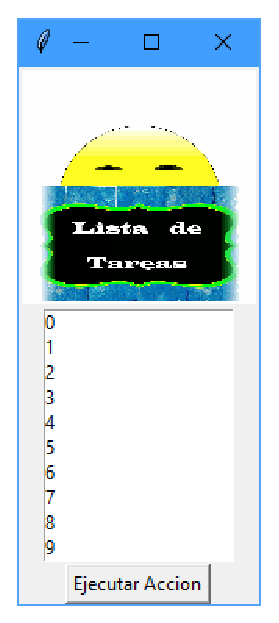
\includegraphics[width=0.2\columnwidth]{chap4/Imagenes/ventana1.eps}
\caption{Ventana principal con el asistente y una lista de tareas
 guardadas.}
\label{fig:v01}
\end{figure} 


Al momento de detectarse una tarea repetitiva, se le muestra al usuario una 
 ventana de captura como se observa en la figura \ref{fig:v02}, en la cual 
 se aprecia al mismo asistente amarillo con otro letrero y la secuencia 
 obtenida, tambi\'en se observa un cuadro de texto para introducir el nombre 
 solicitado, mas abajo se localizan los botones para guardar la tarea y 
 agregarla a la lista de la figura \ref{fig:v01} o ignorarla.}

\begin{figure}[H]
\centering
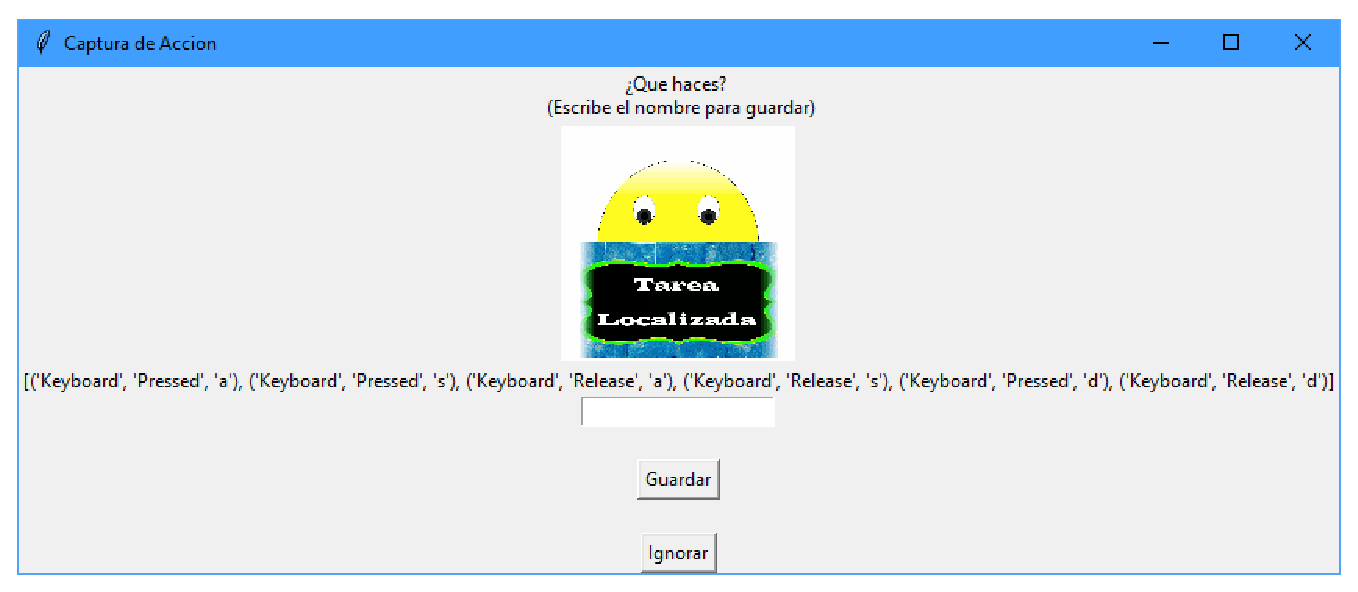
\includegraphics[width=1.0\columnwidth]{chap4/Imagenes/ventana2.eps}
\caption{Ventana mostrando una tarea encontrada.}
\label{fig:v02}
\end{figure}


\end{itemize}

A continuaci\'on se presenta el pseudo--codigo del programa desarrollado.


\begin{table}[]

\begin{lstlisting}

Procedimiento monitoreo
Mientras Verdad Hacer
    Nodo = Capturar accion de teclado o raton
    Si Nodo existe en grafo Entonces
        Incrementar contador_Nodo
    Si no Entonces
        Colocar Nodo en grafo
        Si contador_nodo > 70 Entonces
            Si Nodo existe en Secuencia Entonces
                Si Secuencia existe en Lista_secuencias Entonces
                    Si contador_Secuencia > 5 Entonces
                        Escribir ``Si desea Guardar la tarea 
                                    [Secuencia], escriba un nombre''
                        Leer Respuesta
                        Si Respuesta es nombre Entonces
                            Agregar Secuencia a Lista_Tareas
                        Si no Entonces 
                            Agregar Secuencia a Lista_Ignoradas
                    Si no Entonces
                    Incrementar contador_Secuencia
                Si no Entonces
                    Agregar Secuencia a Lista_Secuencias
            Borrar Secuencia
            Si no Entonces
                Agregar nodo a Secuencia
		Si no Entonces
            Borrar Secuencia
Fin Mientras
Fin Procedimiento 

Procedimiento Ejecucion
Mientras Verdad Hacer
Escribir ``Selecciona la tarea a ejecutar''
Leer Selecci\'on
Escribir ``Ejecutar Accion seleccionada?''
Leer Decisi\'on
Si Decisi\'on = ``Si'' Entonces
	Ejecutar Seleccion
Fin Mientras
Fin Procedimiento

\end{lstlisting}

\end{table}
